
The openETCS tool chain is the implementation of the design process of
the on board unit  (\gls{OBU}) according to the CENELEC EN 50128.
It coordinates the set of tools and methods needed to accomplish this
task and it defines the procedure to follow  to achieve a on board
unit software {\em certifiable} \gls{SIL}4.

Following the proposal of the \cite{D2.3} the tool chain implements
the  life cycle presented figure \ref{fig:lifecycle}.
\begin{figure}
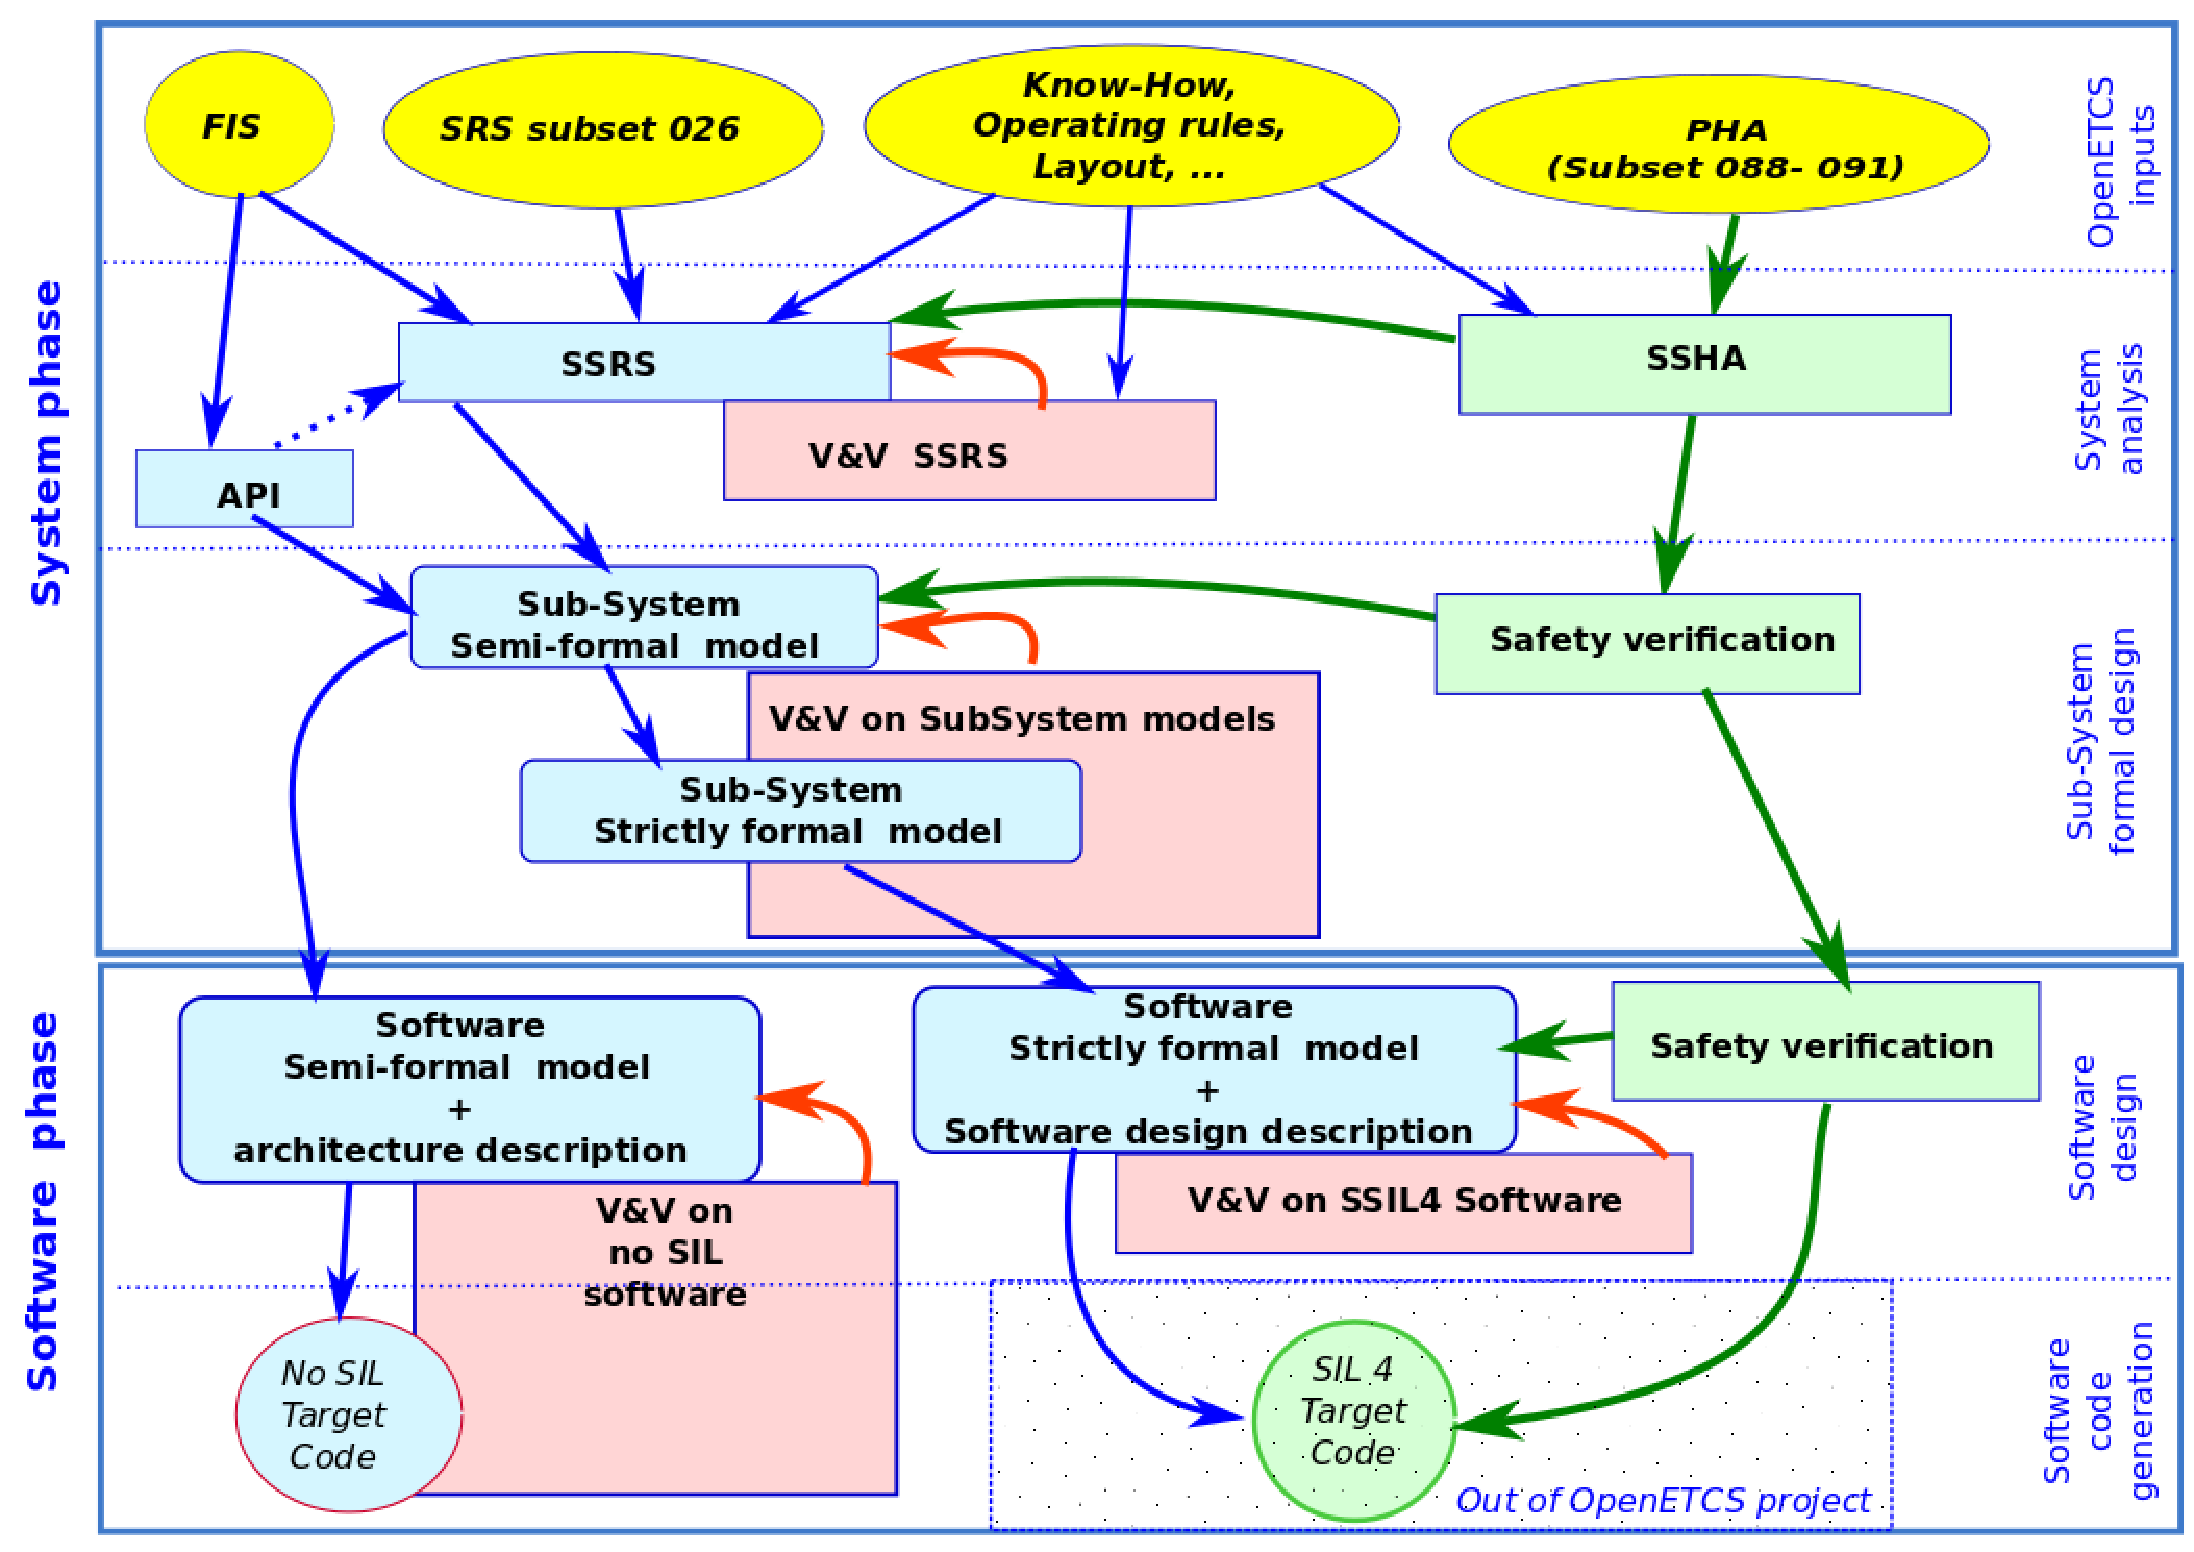
\includegraphics[width=\textwidth]{WholeProcess}
\caption{\label{fig:lifecycle} Life cycle of the on board software}
\end{figure}

Moreover the tool chain should support the activities for producing
certifiable software such as :
\begin{itemize}
\item Software planning
\item Requirements tracing
\item Tool confidences 
\item Documentation/report production
\item Testing 
\item Verification and validation
\end{itemize}

The tool chain should also take care to provide the following
functioning infrastructure to allow robust distributed development
within the defined life cycle. 
\begin{itemize}
\item a continuous automated build system,
\item  mechanisms to upgrade tools in the platform,
\item  mechanisms to add tools to the chain at a later stage (without
  breaking compatibility),
\item modification and change control manager,
\item  tool chain documentation system.
\end{itemize}

Finally the OpenETCS tool chain  should satisfy the requirements of
\cite{D2.6}. Annex A provides a check list of all requirements the
tool chain must fulfill.


%%% Local Variables: 
%%% mode: latex
%%% TeX-master: "WP7-ToolChainDevelpmentPlan"
%%% End: 
